\ifdefined\included
\else
\setcounter{chapter}{5} %% Numéro du chapitre précédent ;)
\dominitoc
\faketableofcontents
\fi

\chapter{Evaluation of Human-Aware Navigation}
\chaptermark{Evaluation of HAN}
\label{chap:6}
\minitoc

\section{Introduction}

%%%%%%%%%%%%% Previous %%%%%%%%%%%%%%%%%
% Evaluating the efficiency and performance of a HAN planning system is one of the open questions in the field. Although there already exists a set of metrics, we believe that these metrics cannot do justice in evaluating a HAN system under intricate scenarios such as the ones addressed in this thesis. Majority of the existing metrics are based on the proxemics violation or some optimality criteria (shortest path, min time etc.) that may not be applicable in case of a robot navigating in a narrow corridor or passage. Therefore, we propose some new metrics for evaluation of HAN in this chapter that can be applied to a wide range of settings.

% Before proposing new metrics, we present some of the generally used metrics in section \ref{ex_metrics} and discuss their limitations. Then we present the proposed metrics in section \ref{new_metrics} along with their mathematical formulation if any. In section \ref{metrics_eval} we test the proposed metrics in different HAN settings and show a detailed analysis. Finally, some conclusions about HAN evaluation metrics are discussed in section \ref{conclude_metrics}.  
%%%%%%%%%%%%% Previous %%%%%%%%%%%%%%%%%

Evaluating the efficiency and performance of a HAN planning system is one of the open questions in the field. Although there are already a set of evaluation metrics, we believe they may not do complete justice to evaluating a HAN system under intricate scenarios such as the ones addressed in this thesis. The majority of the works in HAN evaluate their systems based on the classical navigation metrics combined with proxemics violation. However, proxemics may not be applicable in all scenarios, and sometimes the robot has to intrude into the personal space. Given the circumstances, the human might not feel uncomfortable or even allow it to happen. For example, consider the case of a narrow corridor. Here, both agents have to pass close to each other to reach their goals, and proxemics violations always occur. Therefore, new evaluation metrics that are valid in such situations have to be defined. Some of the existing studies \cite{takayama2009influences, lichtenthaler2012increasing, kruse2014evaluating} talk about how the velocity modulation is more legible and slower speeds are preferred in close vicinity by humans. Therefore, we propose a few new metrics for HAN based on distances, velocities and human visibility which can be applied to a wide range of settings.

Before proposing new evaluation metrics, we present some of the most commonly used evaluation metrics in section \ref{ex_metrics} and discuss some of their shortcomings. Then we present the proposed metrics in section \ref{new_metrics} along with their mathematical formulation, if any. In section \ref{metrics_eval}, we test the proposed metrics in different HAN settings and show a detailed analysis. Finally, some conclusions about HAN evaluation metrics are discussed in section \ref{conclude_metrics}.

\section{Existing Evaluation methods}\label{ex_metrics}
The existing evaluation methods~\cite{gao2021evaluation} and metrics of HAN can broadly be divided into four categories: 1) Navigation metrics, 2) Naturalness metrics, 3) Discomfort metrics and 4) Surveys and studies. We briefly describe each of these categories and present some of the commonly used metrics. Our main focus will be on the discomfort metrics as they deal with the evaluation of human-robot interaction.

\subsection{Navigation Metrics}
All the metrics of navigation can be used to evaluate the navigation performance of a HAN system. They can be used to test the robustness and stability of the designed system and are seldom useful to evaluate the interaction with a human. Some of these metrics are listed here:
\begin{itemize}
    \item \textit{Path Length}: Comparing the length of the path is one of the basic evaluations, and classically, the shorter the path, the better the system. In HAN, however, it may not be true.
    \item \textit{Path Efficiency}: It is the ratio of the distance between two waypoints to the traversed distance between these two waypoints. This measure shows how well the controller is tracking the path.
    \item \textit{Time to reach goal}: It is again one of the simplest metrics which computes the time taken by the robot to reach the final goal. A shorter time is usually preferred, but in HAN, it is not that straightforward. 
    \item \textit{Success Rate}: Success rate is used to quantify the navigation performance and measures how many times the robot navigation was successful over several trials. Irrespective of the type of system, this metric can be applied.
    \item \textit{Number of collisions}: Similar to success rate, counting the number of collisions applies to all navigation systems. Some works in HAN use a modification to measure human safety, called collision index~\cite{truong2014dynamic} and the lower the index, the better.
\end{itemize}

\subsection{Naturalness Metrics}
The naturalness of the robot's trajectory is measured using similarity and smoothness metrics. Similarity metrics measure how similar the robot's trajectory is when it is compared to an expert human trajectory. The smoothness metrics, on the other hand, measure how smooth the robot's motion was during the navigation. Some of these metrics are presented below:
\begin{itemize}
    \item \textit{Path Deviation}: There are different ways in which path deviation is measured. These metrics measure how similar the robot's motion is when compared to an expert trajectory. Two of these ways are:
    \begin{itemize}
        \item \textit{Average Displacement Error (ADE)}: It is the average euclidean distance between the predicted robot's trajectory and the expert (or human) trajectory \cite{pellegrini2009you}. Some works used a non-linear version of this \cite{alahi2016social}.
        \item \textit{Final Displacement Error (FDE)}: It is the distance between the final goal of the predicted trajectory and the given ground-truth data at the same time.
    \end{itemize} 
    \item \textit{Cumulative heading changes}: The changes in the path and the amount of unnecessary turning over the whole path are good metrics to measure the smoothness of the robot's motion. It is also called path irregularity~\cite{guzzi2013human}.
    \item \textit{Acceleration and Velocity}: The motion profiles of the robot can tell us a lot about the smoothness of the trajectory and are some of the basic metrics to use.
    \item \textit{Topological Complexity}: Some works~\cite{mavrogiannis2018social, mavrogiannis2019effects} measure the entanglement in paths using topological complexity index~\cite{dynnikov2007complexity} and use it as a measure of legibility. 
\end{itemize}

The smoothness and topological complexity metrics can be used to measure legibility in HAN systems. Legibility comes with expressiveness, and hence it is necessary to define some metrics for measuring navigation intention expressiveness apart from legibility.

\subsection{Discomfort Metrics}
HAN is essentially a human-robot interaction in the context of robot navigation, and it is necessary to measure how well or how bad the interaction was. Discomfort metrics aim to measure this and tell how well a HAN system is performing. Therefore, these metrics are naturally employed to compare different HAN systems. Most of the existing metrics are distance based and largely rely on the proxemics theory. The most commonly used metrics measure the intrusions into the spatial zones around humans, and some of these are:
\begin{itemize}
    \item \textit{Personal Space Intrusions}: The space surrounding a human is divided into different concentric circles (or other shapes)~\cite{rios2015proxemics} with varying radii defining the proxemics zones. The intrusions into personal and intimate spaces are usually taken as a measure of discomfort, and many works~\cite{okal2016learning, perez2018teaching} count the number of these intrusions to quantify a HAN system. Truong et al.~\cite{truong2017toward} defined a Social Individual Index (SII) based on proxemics (same as collision index in \cite{truong2014dynamic}), and a good HAN system will always have this value below the given threshold. 
    \item \textit{Interaction Space Intrusions}: Similar to individual humans, a group of humans also have various interactions zones like \textit{o-space}, \textit{p-space} and \textit{r-space}~\cite{ferrer2017robot, rios2015proxemics}, and their shape depends on the \textit{f-formation}~\cite{kendon2010spacing} maintained by the members of the group. In such settings, the intrusion into \textit{p-space} and \textit{r-space} are considered as violations and HAN systems try to minimize these intrusions. Sometimes, the human-object interactions are also considered~\cite{truong2017toward} (use Social Group Index (SGI)) while measuring these intrusions.
    \item \textit{Time spent in proxemics zones}: A better alternative to the number of intrusions is to measure the time spent in the areas associated with the human's personal zone or the group's interaction zone~\cite{kostavelis2017robot}.  
    \item \textit{Distance to a human}: While the robot is navigating, there may be different distances from different humans in the environment. In general, HAN systems use either minimum or maximum distance to the closest human and the average distance over all the humans to quantify the system.
\end{itemize}

One of the very useful metrics combining the velocity and distance is called \textit{\acrfull{ttc}}~\cite{biswas2022socnavbench}, and it represents how the robot's motion is relative to the human's motion. The higher the value of \textit{\acrshort{ttc}}, the better the navigation. Truong et al.~\cite{truong2017toward} define something similar called the Relative Motion Index (RMI), and the higher its value, the lower the social acceptance. After checking the formulation, one can notice that RMI is the inverse of \textit{\acrshort{ttc}}. One of the metrics proposed in this chapter is based on \textit{\acrshort{ttc}}, and for this, we provide a detailed description and mathematical formulation in the subsequent sections.

\subsection{Surveys and Studies}
Human interactions and their psychological impressions and states cannot be quantified using just numbers. It requires some well-designed studies and questionnaires, and experimental evaluations on a real system or through videos. HAN does the same to evaluate the psychological safety (discomfort and stress) and the sociability of the system under study. The perceived psychological safety is commonly measured using questionnaires~\cite{butler2001psychological}. Some of the established questionnaires in social robotics like Godspeed~\cite{bartneck2008measuring} already include perceived safety and emotional states and the Robotic Social Attributes Scale (RoSAS) measures several psychological factors based on the Godspeed questionnaire.

The social intelligence of a robot, sometimes called sociability, is not very easy to quantify. A robot's motion may be perfectly natural, satisfies all the comfort based metrics and can still be perceived as not completely social. In several intricate scenarios, the robot might not reach the high level expectations of a human and fail to convey its intention or behaviour to the human. Barchard et al.~\cite{barchardperceived} proposed Perceived Social Intelligence (PSI) scales to evaluate around 20 aspects of the social intelligence of a robot. This was used in some of the recent works~\cite{banisetty2021implicit, barchard2020measuring} to evaluate the HAN system. Some works~\cite{vega2018planning} have employed customs questions apart from these scales to study sociability.

\section{Proposed Discomfort Metrics}\label{new_metrics}
We believe that social space violations by a robot can be permitted to some extent as long as the robot's intentions are conveyed clearly to the human. One of the recent studies by Joosse et al.~\cite{joosse2021making} proposed that people are more lenient when a robot intrudes on their personal space than a human. Further, they showed that these intrusions could be mitigated by conveying the robot's intention to the humans. These studies and observations lay the basis for our metrics based on velocity. The second set of metrics is based on the human's visibility and recognition of the robot when it appears unexpectedly or when it is trying to approach a human for an interaction. We introduce each of these metrics and provide their mathematical formulation in this section.

\subsection{Velocity based Metrics}
Depending on the directions and the magnitudes of the velocities of humans and the robot, we define two metrics (or costs) to evaluate HAN systems. Fig. \ref{fig:vel_metrics} shows two such scenarios where the human and robot can approach each other, or the robot can pass by the human. We define two costs to assess such situations namely, 1) $cost_{danger}$ and 2) $cost_{passby}$. The idea behind $cost_{danger}$ is to evaluate how fast a robot moves directly towards the human causing discomfort and, in some cases, fear. This is primarily associated with the danger of collision, hence the name $cost_{danger}$. If something or someone passes at a very high speed in close vicinity, it could lead to confusion or discomfort. The second metric, $cost_{passby}$, could be used to evaluate how the HAN system handles such scenarios. We now proceed to the details and the mathematical formulations of these costs.
\begin{figure}[!h]
    \centering
    \includegraphics[width=0.9\columnwidth]{images/chapter6/vel_metrics.pdf}
    \caption{Human-Robot situations where velocity based metrics are important. (a) Cross: The human and the robot are approach and cross each other with different velocities. (b) Overtake or Follow: The robot is behind the human and is about to overtake or follow the human. In both the situations, the human can be either static or moving but the robot is always moving.}
    \label{fig:vel_metrics}
\end{figure}

\subsubsection{Formulation}
Suppose the circumscribed circle of the human has a radius of $r_h$ and that of the robot has a radius of $r_r$. The human and the robot collide when the distance between their centres is less than or equal to the sum of these radii, $r_h+r_r = R$. If we assume the robot is a point and expand the radius of the human to $R$, the same conditions apply. This setting is shown in Fig. \ref{fig:vel_vectors} along with the velocities of the human, $\overrightarrow{V_h}$ and the robot, $\overrightarrow{V_r}$. 
\begin{figure}[h!]
    \centering
    \includegraphics[width=0.9\columnwidth]{images/chapter6/fig_vector.pdf}
    \caption{Mathematical Formulation of the costs. The figure shows the different vectors and the possible costs depending on the situation. If $\overrightarrow {V_{rel}}$ falls within the zone indicated by the dotted lines then there is $cost_{danger}$ and if it falls outside this zone then we have the $cost_{passby}$. Human's velocity is represented by $\overrightarrow{V_h}$, robot's velocity by $\overrightarrow{V_r}$, the position vector from the robot to the human by $\overrightarrow{P_{rh}}$. $\theta$ is the angle between $\overrightarrow{V_{rel}}$ and $\overrightarrow{P_{rh}}$. Note that only one of the $\overrightarrow{V_{rel}}$ (blue or red one) exists at a time, but not both.}
    \label{fig:vel_vectors}
\end{figure}
The relative velocity of the robot with respect to the human is given by $\overrightarrow{V_{rel}}=\overrightarrow{V_r} - \overrightarrow{V_h}$ and depending on where it falls (see Fig. \ref{fig:vel_vectors}), we define two types of metrics or costs. If it falls within the collision zone, represented by dotted lines, then there is a danger of collision, and hence, we define the $cost_{danger}$ in this setting. If it falls outside the collision zone, the danger of collision no longer exists, but the robot may pass by the human, and so in this setting, we define the $cost_{passby}$. Let the vector from the robot's position to the human's position be $\overrightarrow{P_{rh}}$ and $\theta$ be the angle between $\overrightarrow{V_{rel}}$ and $\overrightarrow{P_{rh}}$. While defining these costs, we use the effective distance between the human and the robot, $d_{rh_{eff}}$ and the perpendicular component of $\overrightarrow{P_{rh}}$ along $\overrightarrow{V_{rel}}$, $d_{\perp}$. 


\subsubsection{Metrics}
The first of the two metrics is the cost of danger when there is a possibility of collision. This metric can be seen as a measure of the feeling of threat a robot can cause while it moves directly towards the human. For this, we use first calculate the $\acrshort{ttc}$ based on the above formulation,
\begin{equation*}
\centering
\begin{multiline*}
    TTC = \frac{d_{rh_{eff}}}{\lVert \overrightarrow{V_{rel}} \rVert} = 
    \frac{\overrightarrow{P_{rh}}\cdot\overrightarrow{V_{rel}}
    - \sqrt{\left(\overrightarrow{P_{rh}}\cdot\overrightarrow{V_{rel}}\right)^2 
    - \left(\left\lVert \overrightarrow{V_{rel}} \right\rVert^2 
        \left( \left\lVert \overrightarrow{P_{rh}} \right\rVert^2 - R{^\strut{2}} \right) \right)}}{\left\lVert \overrightarrow{V_{rel}} \right\rVert^2}\\
        
        when \overrightarrow{P_{rh}}\cdot\overrightarrow{V_{rel}} >0\ \text{and}\ \left(\overrightarrow{P_{rh}}\cdot\overrightarrow{V_{rel}}\right)^2 
    - \left(\left\lVert \overrightarrow{V_{rel}} \right\rVert^2 
        \left( \left\lVert \overrightarrow{P_{rh}} \right\rVert^2 - R{^\strut{2}} \right) \right) > 0
\end{multiline*}
\end{equation*}

\noindent where `($\lVert \rVert$)' is the magnitude of the vector and `$(\cdot$)' is the dot product. Note that $TTC$ is only defined when the $\overrightarrow{V_{rel}}$ falls within the collision zone. Outside this zone, $TTC = \infty$. When $TTC>0$, the cost of danger is defined as follows,
\begin{equation}
    cost_{danger} = \frac{1}{TTC} = \frac{\lVert \overrightarrow{V_{rel}} \rVert}{d_{rh_{eff}}}
\end{equation}

When the $\overrightarrow{V_{rel}}$ falls outside the collision zone, the $cost_{danger}=0$ and as $\lvert\theta\rvert$ or $d_{rh_{eff}}$ decreases or $\lVert \overrightarrow{V_{rel}} \rVert$ increases, $cost_{danger}$ increases. Any HAN system can be defined to have a certain threshold for this cost beyond which some mitigating actions have to be taken. The second metric that we propose is valid when $\overrightarrow{V_{rel}}$ is outside the collision zone. In such a setting, the robot may follow or pass by the human, and we define the $cost_{passby}$ as,
\begin{equation}
    \begin{gathered}
    \centering
    cost_{passby} = \frac{\lVert \overrightarrow{V_{rel}} \rVert}{d_{\perp}-R}\lvert sin(\theta) \rvert \\
    &= \frac{\left\lVert \overrightarrow{V_{rel}} \right\rVert\left\lvert \sqrt{\left\lVert \overrightarrow{V_{rel}} \right\rVert^2 \left\lVert \overrightarrow{P_{rh}}\right\rVert^2-\left(\overrightarrow{P_{rh}}\cdot\overrightarrow{V_{rel}}\right)^2}\right\rvert}{\left\lVert \overrightarrow{P_{rh}} \right\rVert \left( \sqrt{\left\lVert \overrightarrow{V_{rel}} \right\rVert^2 \left\lVert \overrightarrow{P_{rh}} \right\rVert^2-\left(\overrightarrow{P_{rh}}\cdot\overrightarrow{V_{rel}}\right)^2}-\lVert \overrightarrow{V_{rel}} \rVert R \right)}\\
\end{gathered}    
\end{equation}
when $\overrightarrow{P_{rh}}\cdot\overrightarrow{V_{rel}} >0$ and $d_{\perp}>R \implies  \sqrt{\left\lVert \overrightarrow{V_{rel}} \right\rVert^2 \left\lVert \overrightarrow{P_{rh}} \right\rVert^2-\left(\overrightarrow{P_{rh}}\cdot\overrightarrow{V_{rel}}\right)^2} >\lVert \overrightarrow{V_{rel}} \rVert R$. The $cost_{passby}$ increases as the robot approaches the human. Specifically, the cost increases as the perpendicular distance of the robot from the human decreases or the relative velocity increases. It also increases as $\theta$ increases, indicating that the robot is getting closer to the human. The main idea behind this metric is that a robot passing very close to a human at a very high speed could cause discomfort to the human.

\subsection{Vision based Metrics}
A human moving in an environment depends on different senses to identify and negotiate the path or the moving direction. In such conditions, if something or someone appears suddenly without any intimation, the human might be surprised, and sometimes he/she might not even feel comfortable with such appearances. This applies to static humans as well. We believe that in the case of static humans, the robot has to maintain a larger distance behind the human~\cite{avrunin2014socially} to avoid causing any discomfort or surprise. Moreover, when the robot is planning to enter a human's field of view (FoV), it should enter at a convenient distance and angle to avoid any compensatory actions by the human. An illustration of such conditions is provided in Fig. \ref{fig:vis_metrics}. The depiction on the left shows a robot trying to enter the human's FoV for interaction, and the one on the right shows the sudden appearance of a robot in front of the human without having any knowledge about the whereabouts of the human.

\begin{figure}[!h]
    \centering
    \includegraphics[width=0.9\columnwidth]{images/chapter6/vision_metrics.pdf}
    \caption{Human-Robot interaction scenarios where vision based metrics are needed apart from velocity based ones. (a) Approach: The robot is approaching human for an interaction. The robot needs to go from the back to the front to initiate the interaction. (b) Appear: The robot and human suddenly face each other without any prior knowledge about the other. The human can be static or dynamic in both these settings.}
    \label{fig:vis_metrics}
\end{figure}

Considering all these, we propose $cost_{visibility}$, $cost_{surprise}$ and $cost_{react}$ to evaluate such situations. The first one, $cost_{visibility}$, measures how visible the robot is when it enters the FoV of a human below a certain threshold distance. The idea is to evaluate how well the HAN system adapts to the visibility of the robot. $cost_{surprise}$, on the other hand, measures how surprised or uncomfortable a human is when a robot appears suddenly in a human's FoV, whereas $cost_{react}$ measures how safe the appearance is. These metrics are designed to evaluate how well a HAN system handles sudden or occluded emergences of humans.  

\subsubsection{Formulation}
In this formulation as well, we consider the robot as a point, and the circumscribed radius of the human is taken as $R=r_h+r_r$. The vector from the human's position to the robot's position is represented by $\overrightarrow{P_{rh}}$, and the unit vector in the direction of orientation of the human is given by $\hat{u}_h$.
\begin{figure}[!h]
    \centering
    \includegraphics[width=0.8\columnwidth]{images/chapter6/fig_vision_2.pdf}
    \caption{Mathematical formulation for vision-based metrics. $\theta$ is the angle between the unit vector of human's direction, $\hat{u}_h$ and vector $\overrightarrow{P_{hr}}$. $\theta_{FoV/2}$ is the half angle of human's field of view and $d_{hr_{eff}}$ ($= \left\lVert \overrightarrow{P_{hr}} \right\rVert - R$) is the effective distance between the human and the robot.}
    \label{fig:vision_vectors}
\end{figure}
The angle between $\overrightarrow{P_{rh}}$ and $\hat{u}_h$ is represented by $\theta$ and the half angle of human's FoV by $\theta_{FoV/2}$. The effective distance between the human and the robot is given by $d_{hr_{eff}}$. When the robot comes into the FoV of the human (green area in the figure), we define three costs using $d_{hr_{eff}}$, $\theta$ and some studies based on human perception.
\subsubsection{Metrics}
We first define the visibility cost, $cost_{visibility}$ as follows,
\begin{equation}
    \begin{gathered}
        cost_{visibility} = \frac{d_{proxemics}}{d_{hr_{eff}}}\left(\frac{\theta}{\theta_{FoV/2}}\right) = \alpha\left( \frac{cos^{-1}\left(\hat{u}_h\cdot\overrightarrow{P_{hr}}\right)}{\left\lVert \overrightarrow{P_{hr}} \right\rVert\left( \left\lVert \overrightarrow{P_{hr}} \right\rVert - R\right)}\right)\\
        % = \frac{d_{proxemics}}{\theta_{FoV/2}}\left(\frac{cos^{-1}\left(\hat{u}_h\cdot\overrightarrow{P_{hr}}\right)}{\left\lVert \overrightarrow{P_{hr}} \right\rVert\left( \left\lVert \overrightarrow{P_{hr}} \right\rVert - R\right)}\right)\\
    \end{gathered}
\end{equation}
where $\alpha = \frac{d_{proxemics}}{\theta_{FoV/2}}$ and $d_{proxemics}$ is the defined proxemics based distance that do not intrude the personal space ($> \SI{0.45}{\metre}$). The lesser the cost of visibility, the better the behaviour of the robot. This cost increases as $\theta$ increases indicating that more human effort is needed to look at the robot (head motion). The cost also increases as the distance, $d_{hr_{eff}}$, decreases to discourage close and sudden appearances.

When a human sees something, it takes a few milliseconds before it is registered by the brain. After the recognition, it takes more time to generate a response. The average recognition time for a human is around $t_{recognise}= 150$ milliseconds~\cite{thorpe1996speed, rayner2009eye} and the average time to react for visual stimuli is between $t_{react}=400-600$ milliseconds~\cite{eckner2012novel, wolfe2020rapid}. If something appears very close to a human before it can be recognised, it could result in a surprise or shock. Even after recognition, if there is no time to respond, it could result in a collision or may cause discomfort. Taking all of this into account, we propose two costs to measure surprise and response based on the robot's position when it appears. They follow similar formulations with some differences. We first define a linearly increasing function called the `seen ratio' ($SR$) as given below,
\begin{equation}
    SR  = \begin{cases}
       \frac{t}{t_{react}},\ &\quad\text{if} \ 0<t<t_{react}\\
       1,&\quad\text{if} \ t\geq t_{react}\\
     \end{cases}
\end{equation}
% \begin{figure}[!h]
%     \centering
%     \includegraphics[width=0.7\columnwidth]{images/chapter6/SR_plot.pdf}
%     \caption{Seen Ratio ($SR$) as a function of time.}
%     \label{fig:sr_plot}
% \end{figure}

SR starts at zero the moment the robot enters the human's FoV, and as time, $t$, passes, this ratio slowly increases until it reaches one. When the value of $SR$ is one, it means that the robot has been seen and identified by the human with enough time to react if needed. Hence, we can say that the $SR$ becomes one at around $t = t_{react} = 600$ milliseconds and continues to stay at one until the robot moves out of FoV of the human. The costs are defined as follows,

\begin{align}
    cost_{surprise} &=max\left(\frac{d_{proxemics}}{d_{hr_{eff}}}(1-\gamma SR) , 0\right)\\
    cost_{react} &= \frac{d_{proxemics}}{d_{hr_{eff}}}\left(1-SR\right)
\end{align}

where $\gamma = \frac{t_{react}}{t_{recognise}}$. Both $cost_{surprise}$ and $cost_{react}$ are high if the effective distance, $d_{hr_{eff}}$, is low when the robot enters the FoV of the human. $cost_{surprise}$ lasts only for a short period, and if the robot comes very close to a human during this period, the human can be marked as surprised with a corresponding cost. The $cost_{react}$ measures how the robot's appearance affects the human. If the $cost_{react}$ is high, that means the HAN system has done a poor job in handling sudden appearances, and it needs to be improved.  

For all the costs (metrics) proposed, it is ideal to set a threshold below which the behaviour is acceptable, and these can be obtained based on real-world demonstrations and studies. However, such studies are yet to be performed, and therefore, we can only have a relative analysis with respect to another planner. In the next section, we do this comparative analysis using the standard ROS Navigation Stack and \acrshort{cohan}.

\section{Analysis}\label{metrics_eval}
The proposed metrics are used to evaluate four human-robot interaction scenarios given in figures~\ref{fig:vel_metrics} and \ref{fig:vis_metrics} i.e., 1) Cross (Fig. \ref{fig:vel_metrics} a): the human and robot cross each other face-to-face, 2) Follow and Overtake (Fig. \ref{fig:vel_metrics} b): the robot follows and then overtakes a slow-moving human, 3) Approach (Fig. \ref{fig:vis_metrics} a): the robot moves from the back to the front of a static human for interaction and 4) Appear (Fig. \ref{fig:vis_metrics} b): the human suddenly appears as the robot is taking an L-turn. 

In all the experiments, $d_{proxemics}=\SI{1.6}{\metre}$, $\theta_{FoV}=120^\circ$ and $r_h = \SI{0.3}{\metre}$. The interactions are simulated in the MORSE simulator, and the human agent is controlled using InHuS~\cite{favier2021intelligent}. The robot is controlled using two different systems, \acrshort{cohan} and Simple Move Base (SMB). SMB uses the standard ROS navigation stack and adds humans as obstacles. It neither uses human motion prediction nor social norms while navigating. Hence, we expect our metrics to differentiate clearly between SMB and \acrshort{cohan}. Each scenario was run 5 times using both the planners and the mean values of the metrics are tabulated in Table~\ref{evaluation_cross}. In this section, we analyse each of the above four scenarios in detail using these metrics.  
\begin{table*}[!h]
    \centering
    \begin{tabular}{|c|c|c|c|c|c|}
    \hline
     & \multicolumn{5}{c|}{Cross} \\
    \cline{2-6}
    Planner & $cost_{danger}$ & $cost_{passby}$ & $cost_{visibility}$ & $cost_{surprise}$ & $cost_{react}$ \\
    \hline
    \textbf{CoHAN} &\textbf{0.18} &\textbf{1.71} &0.0 &0.0 &0.0 \\ 
    \hline
    \textbf{SMB} &1.19 &9.5 &0.0 &0.0 &0.0 \\
    \hline
    & \multicolumn{5}{c|}{Follow and Overtake} \\
    \cline{1-6}
        \textbf{CoHAN} &0.31 &\textbf{0.90} &\textbf{1.21} &\textbf{0.98} &\textbf{1.19} \\ 
    \hline
    \textbf{SMB} &\textbf{0.27} &0.92 &2.66 &2.15 &2.61 \\
    \hline
    & \multicolumn{5}{c|}{Approach} \\
    \cline{1-6}
        \textbf{CoHAN} &\textbf{0.28} &\textbf{1.05} &\textbf{2.27} &\textbf{1.91} &\textbf{2.32} \\ 
    \hline
    \textbf{SMB} &0.31 &1.95 &3.53 &3.01 &3.66 \\
    \hline
    & \multicolumn{5}{c|}{Appear} \\
    \cline{1-6}
        \textbf{CoHAN} &\textbf{1.46} &7.22 &\textbf{0.49} &\textbf{0.70} &\textbf{0.85} \\ 
    \hline
    \textbf{SMB} &3.15 &\textbf{2.27} &0.77 &0.91 &1.11 \\
    \hline
    \end{tabular}
    \caption{Proposed discomfort metrics in four different scenarios. SMB and CoHAN were run 5 times in each of the scenarios, and the mean values are presented.}
    \label{evaluation_cross}
\end{table*}

\subsection{Scenario 1: Cross}
In this scenario, the robot is already in the FoV of the human as it starts moving. So, all the vision-based metrics will be zero, and only the velocity based metrics are relevant here. Comparing the values of $cost_{danger}$ and $cost_{passby}$ from Table~\ref{evaluation_cross}, the costs corresponding to \acrshort{cohan} are significantly lower than costs for SMB. As \acrshort{cohan} is a human-aware planner, it tries to provide more ways for the human by moving away as shown in Fig.~\ref{fig:paths_cross} (b) and thanks to the \textit{Relative Velocity} constraint, it even slows down as it passes by the human. These behaviours result in low $cost_{danger}$ and $cost_{passby}$. On the other hand, SMB does not modulate its velocity much and takes only a small deviation to avoid the collision, as shown in Fig.~\ref{fig:paths_cross} (a). The slight decrease in human speed and the path change can be seen in Fig.~\ref{fig:paths_cross} (a). Sometimes, the human took the full burden of avoiding the collision. These behaviours may not be acceptable, and it is reflected by the high values in $cost_{danger}$ and $cost_{passby}$.

\begin{figure}[h!]
\centering
\hspace{-0.15cm}
\begin{subfigure}{.5\columnwidth}
  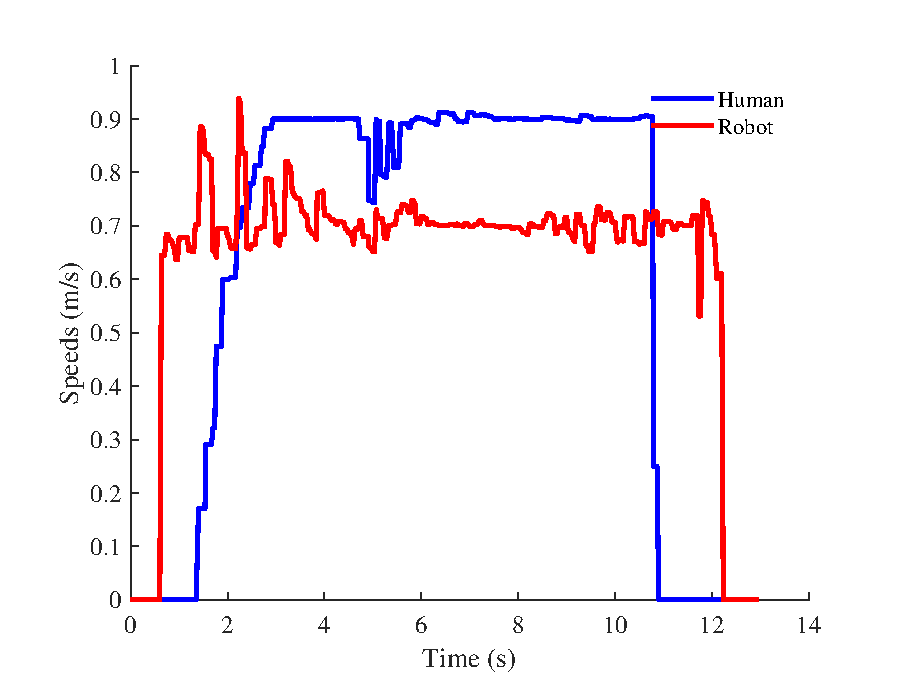
\includegraphics[width=\textwidth]{images/chapter6/smb/cross_vel.eps}
%   \caption{SMB}
\end{subfigure}
\hspace{-0.75cm}
\begin{subfigure}{.5\columnwidth}
  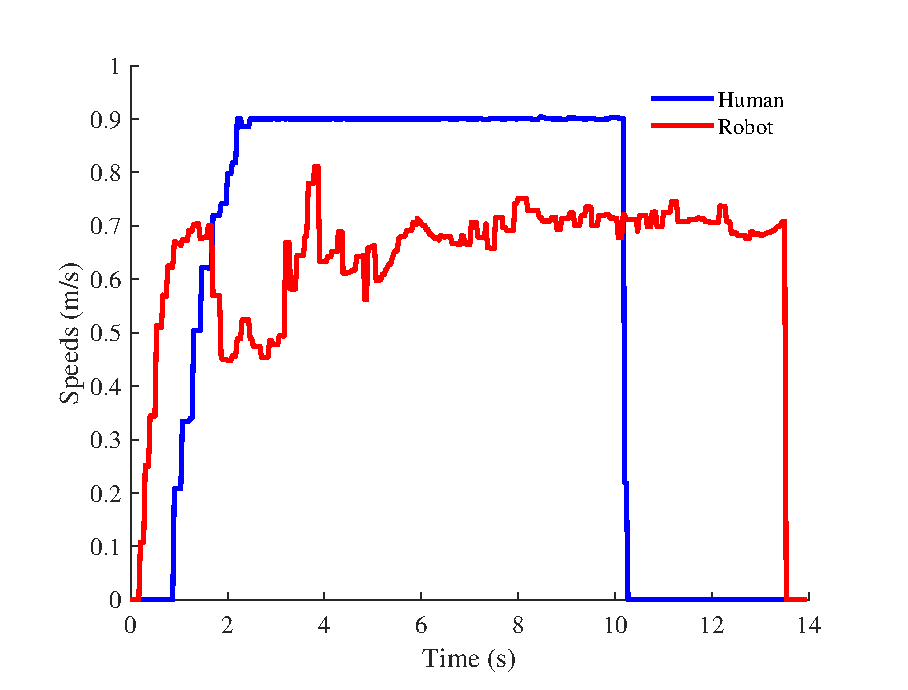
\includegraphics[width=\textwidth]{images/chapter6/cohan/cross_vel.eps}
%   \caption{CoHAN}
\end{subfigure}
\vspace{0.15cm}
\begin{subfigure}{.45\columnwidth}
  \includegraphics[width=\textwidth]{images/chapter6/smb/cross.png}
  \caption{SMB: Cross}
\end{subfigure}
\hspace{0.15cm}
\begin{subfigure}{.45\columnwidth}
  \includegraphics[width=\textwidth]{images/chapter6/cohan/cross.png}
  \caption{CoHAN: Cross}
\end{subfigure}
\caption{Speeds and paths of the human and robot in the Cross scenario. The triangle with the thick line is the human, and the other one is the robot. Both the human and robot move from the blue end to the red end of the paths. (a) In the case of SMB, the robot moves close to the human, and the human path is slightly modified. As they cross each other, there is a slight decrease in the velocity of the human. (b) The robot running CoHAN moves away showing the intention and also keeping its distance from the human. So the human path is almost a straight line, and the velocity remains constant.}
\label{fig:paths_cross}
\end{figure} 

\subsection{Scenario 2: Follow and Overtake}
As explained above, the robot starts following a slow-moving human and finally overtakes him before reaching its goal (Fig.~\ref{fig:paths_follow}). In this situation, a HAN system should have small values for all of the proposed metrics as the robot should pass by the human without colliding and not surprise the human as it overtakes him. From the values of the metrics in the table, it is evident that \acrshort{cohan} performs comparatively better than SMB. Specifically, $cost_{surprise}$, $cost_{react}$ and $cost_{visibility}$ are significantly high for SMB, indicating that the robot might have entered a human's FoV suddenly and at a closer distance which is not ideal. This is true as one can see from Fig~\ref{fig:paths_follow} (a) that the robot was very close as it overtook the human. The robot using \acrshort{cohan} modifies its trajectory to accommodate the \textit{Visibility} constraint and enters the human's FoV in a better manner, as seen in Fig.~\ref{fig:paths_follow} (b). However, we cannot claim that this is the best, as thresholds and benchmarks still need to be set. 

In this setting, the robot and the human have some perpendicular offset distance, unlike in the previous case, and they move almost parallelly for the most part (see Fig.~\ref{fig:paths_follow}). As a result, both SMB and \acrshort{cohan} have similar $cost_{danger}$ and $cost_{passby}$. The $cost_{passby}$ is slightly lower for \acrshort{cohan} because of the velocity modulation, and $cost_{danger}$ is slightly higher because of the directional changes imposed by different constraints. The robot with SMB moves in a straight line, and when it is very close to the goal, it changes its path slightly. 

\begin{figure}[h!]
\centering
\hspace{-0.15cm}
\begin{subfigure}{.5\columnwidth}
  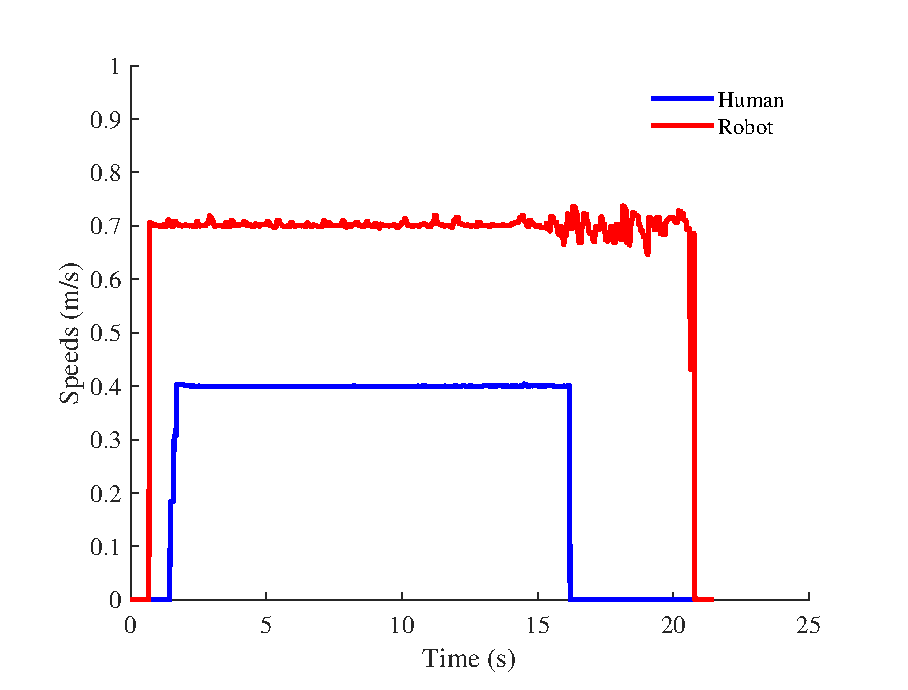
\includegraphics[width=\textwidth]{images/chapter6/smb/overtake_vel.eps}
%   \caption{SMB}
\end{subfigure}
\hspace{-0.75cm}
\begin{subfigure}{.5\columnwidth}
  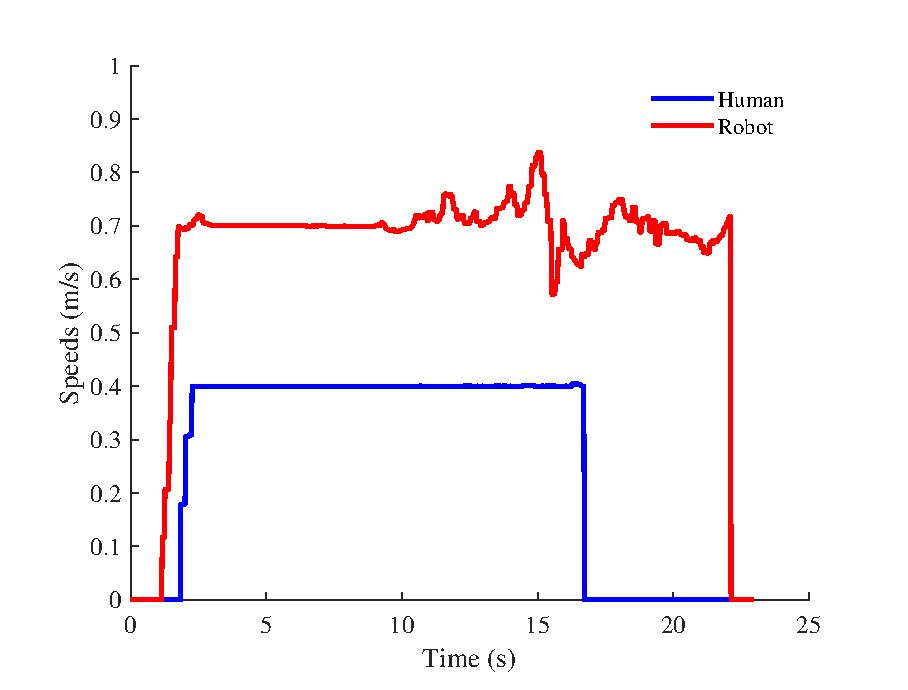
\includegraphics[width=\textwidth]{images/chapter6/cohan/overtake_vel.eps}
%   \caption{CoHAN}
\end{subfigure}
\vspace{0.15cm}
\begin{subfigure}{.45\columnwidth}
  \includegraphics[width=\textwidth]{images/chapter6/smb/follow.png}
  \caption{SMB: Follow and Overtake}
\end{subfigure}
\hspace{0.15cm}
\begin{subfigure}{.45\columnwidth}
  \includegraphics[width=\textwidth]{images/chapter6/cohan/follow.png}
  \caption{CoHAN: Follow and Overtake}
\end{subfigure}
\caption{Speeds and paths of the human and robot in the Follow and Overtake scenario. The triangle with the thick line is the human, and the other one is the robot. Both the human and robot move from the blue end to the red end of the paths. (a) The human and the robot move parallely until the very end without much change in their velocity profiles.(b) The robot with \acrshort{cohan} takes a larger deviation as it plans to enter the FoV of the human. The velocity of the robot drops slightly when it over takes the human and then it increases slowly.}
\label{fig:paths_follow}
\end{figure}

\subsection{Scenario 3: Approach}
\begin{figure}[h!]
\centering
\hspace{-0.15cm}
\begin{subfigure}{.5\columnwidth}
  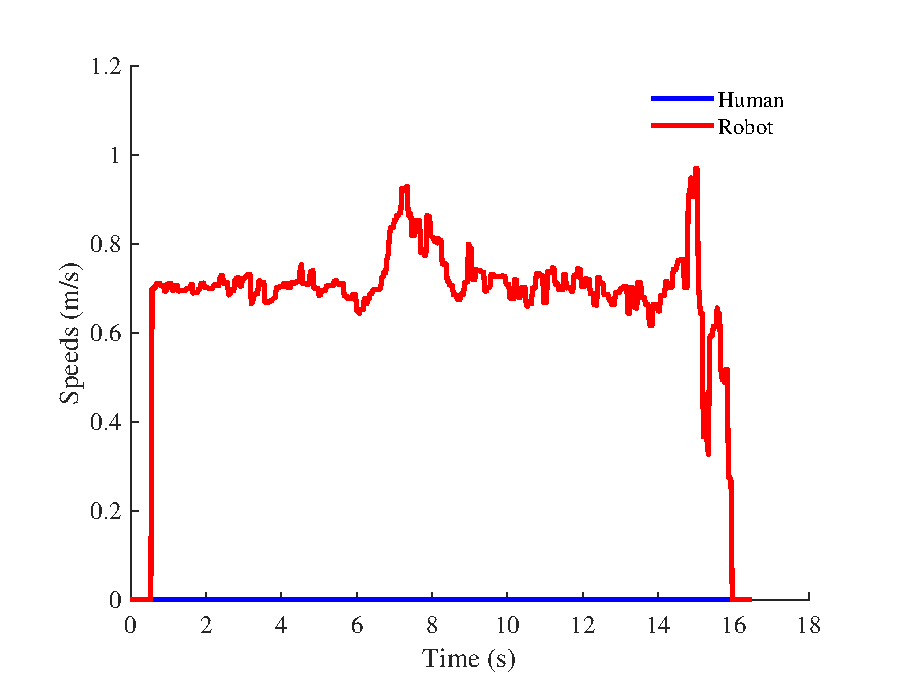
\includegraphics[width=\textwidth]{images/chapter6/smb/approach_vel.eps}
%   \caption{SMB}
\end{subfigure}
\hspace{-0.75cm}
\begin{subfigure}{.5\columnwidth}
  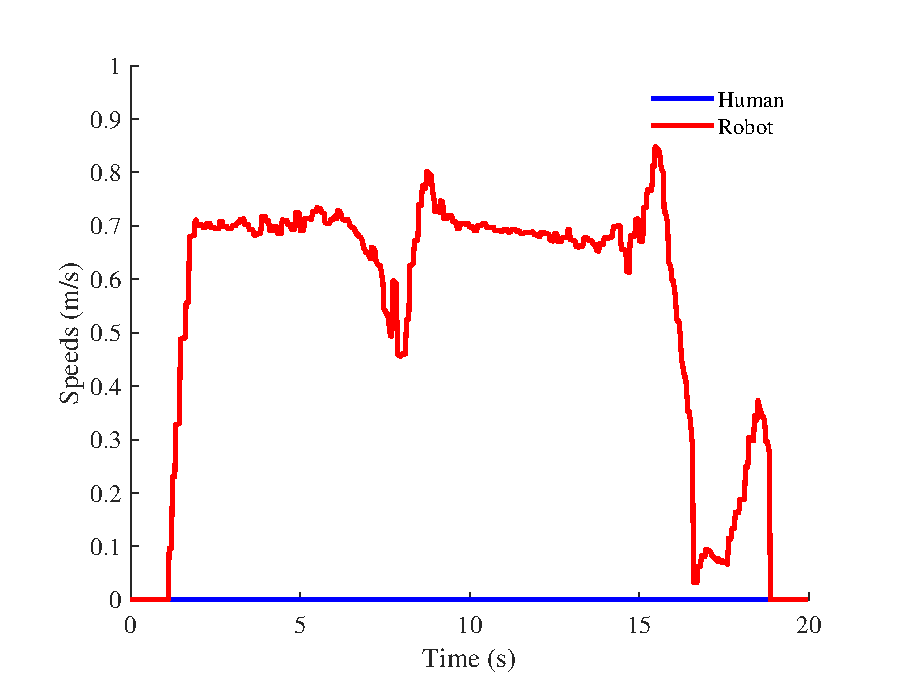
\includegraphics[width=\textwidth]{images/chapter6/cohan/approach_vel.eps}
%   \caption{CoHAN}
\end{subfigure}
\vspace{0.15cm}
\begin{subfigure}{.45\columnwidth}
  \includegraphics[width=\textwidth]{images/chapter6/smb/approach.png}
  \caption{SMB: Approach}
\end{subfigure}
\hspace{0.15cm}
\begin{subfigure}{.45\columnwidth}
  \includegraphics[width=\textwidth]{images/chapter6/cohan/approach.png}
  \caption{CoHAN: Approach}
\end{subfigure}
\caption{Speeds and paths of the human and robot in the Approach scenario. The triangle with the thick line is the human, and the other one is the robot. The robot moves from the blue end to the red end of the paths, and the human is static in the scenario. (a) The robot's path does not deviate much except at the end. (b) The robot's path slightly deviates as soon as the robot sees the human, and when the robot turns itself to align in the close vicinity of the human, CoHAN tries to keep the robot's velocity low.}
\label{fig:paths_approach}
\end{figure}
This is a fairly simple setting with a static human. The robot has to approach and face this static human for interaction. The robot starts somewhere behind the human and has to slowly enter his FoV, reducing the surprise as much as possible. As expected, \acrshort{cohan} has comparatively lower values for all the metrics and in fact $cost_{danger}$ and $cost_{passby}$ are similar to the previous case (Table \ref{evaluation_cross}). Although the vision-based metrics are significantly lower for \acrshort{cohan} than SMB, their values are doubled compared to the \textit{Follow and Overtake} case. This could mean that \acrshort{cohan} has to improve its handling of static humans. The paths and the velocity profiles of the robot are shown in Fig.~\ref{fig:paths_approach}, and we can see that \acrshort{cohan}'s path has slightly deviated, and the robot takes a larger turn. The speed profile in Fig.~\ref{fig:paths_approach} (b) shows that the robot moves with lower velocities while aligning itself in front of the human.

\subsection{Scenario 4: Appear}
When the robot navigates in an environment, there could be several places from where a human can emerge, as discussed in Chapter~\ref{chap:5}. One such scenario is an L-turning, where a robot can find itself facing a previously unseen human suddenly. It is one of the most difficult cases to handle for a HAN system, as it has to prevent harm and shock to the human on top of avoiding the robot from freezing. As \textit{invisible humans} are already a part of \acrshort{cohan}, it is expected to perform better in this case.

From Table~\ref{evaluation_cross}, we can see that \acrshort{cohan} reduces the surprise and has a lesser reaction cost ($cost_{react}$) as well, indicating slightly better performance compared to SMB. The $cost_{danger}$ also indicates the same in comparison with SMB, but the numerical values are high compared to all the previous cases. As the robot was modulating only its path to handle a sudden emergence, the high velocity explains the higher value. With SMB, it is even higher as it does not even modulate its path. The most important metric to discuss in this scenario is the $cost_{passby}$. Looking at the numerical values, it seems like \acrshort{cohan} is performing very bad, and SMB has a better performance. It means that the relative velocity between the human and the robot is high in the case of \acrshort{cohan}.

\begin{figure}[h!]
\centering
\hspace{-0.15cm}
\begin{subfigure}{.52\columnwidth}
  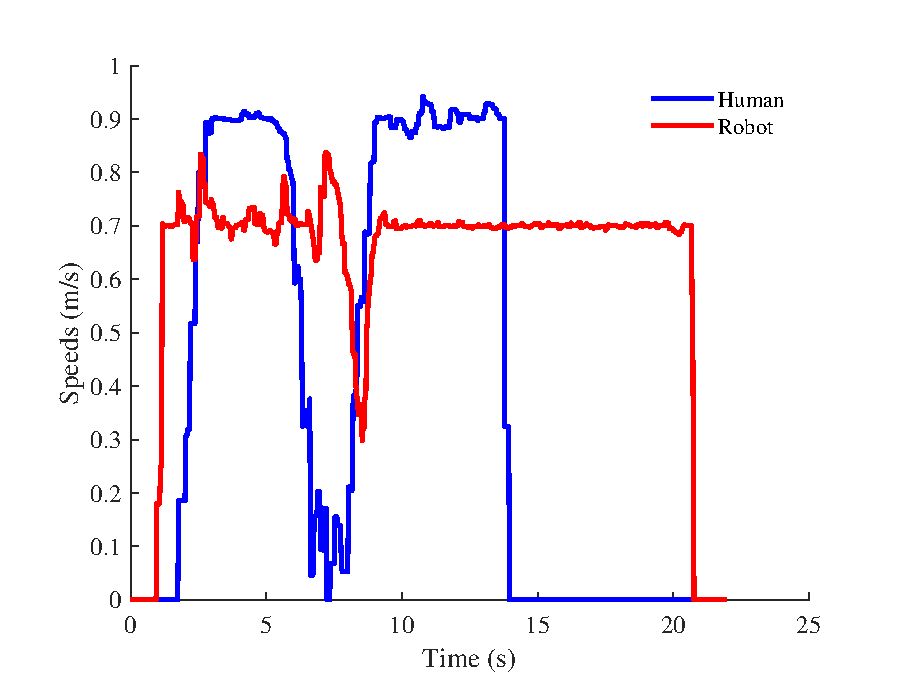
\includegraphics[width=\textwidth]{images/chapter6/vel_smb.eps}
\end{subfigure}
\hspace{-0.75cm}
\begin{subfigure}{.52\columnwidth}
  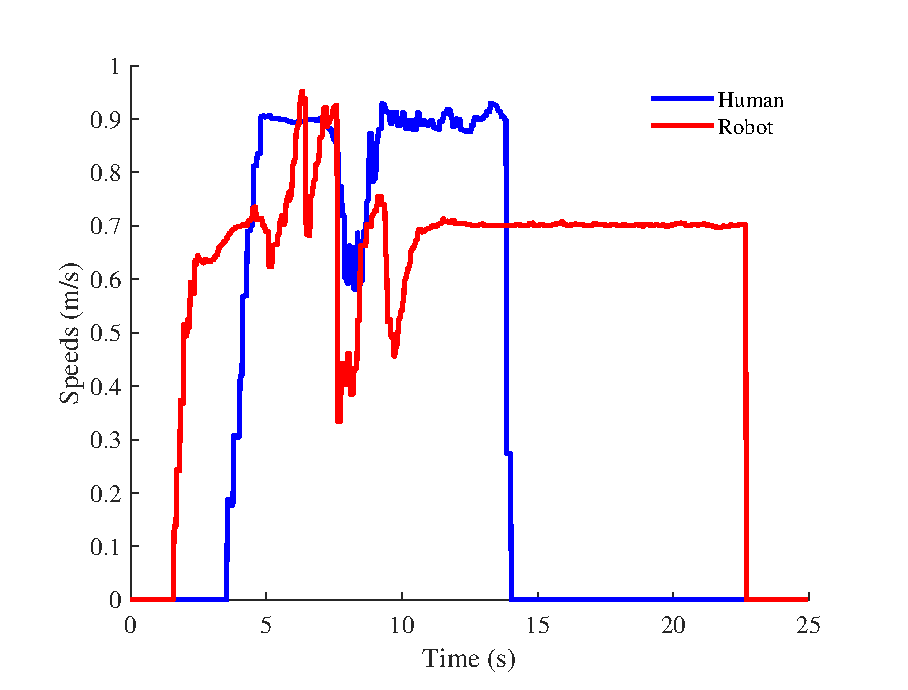
\includegraphics[width=\textwidth]{images/chapter6/vel_cohan.eps}
\end{subfigure}
\begin{subfigure}{.45\columnwidth}
  \includegraphics[width=\textwidth]{images/chapter6/smb/appear2.png}
  \caption{SMB: Appear}
\end{subfigure}
\hspace{0.15cm}
\begin{subfigure}{.45\columnwidth}
  \includegraphics[width=\textwidth]{images/chapter6/cohan/appear.png}
  \caption{CoHAN: Appear}
\end{subfigure}
\caption{Speeds and paths of the human and robot in the Appear scenario. The triangle with the thick line is the human, and the other one is the robot. Both the human and robot move from the blue end to the red end of the paths. (a) The speed of the human drastically changes and momentarily the human even halts as the robot faces him (red circle on path). (b) The robot moves away from the corner and takes the turn with larger radius so that the human does not have to slow down much. The robot speeds up a little to move further away as it sees the human and then slows down while it passes by him.}
\label{fig:vel_plots}
\end{figure}    

The speeds and paths of the human and the robot for SMB and \acrshort{cohan} are shown in Fig.~\ref{fig:vel_plots}. From the speed plots of SMB in Fig.~\ref{fig:vel_plots} (a), we can see that the human's speed drastically falls between $5$ and $10$ seconds, and momentarily, it is even zero. At the same time, the robot's speed seems to be dropping too. This happens as the robot and human face each other, and the robot blocks the human's way (red circle on the path in Fig.~\ref{fig:vel_plots} (a)) before changing its trajectory. This results in a lower relative velocity, and hence, $cost_{passby}$ is small. However, this is not acceptable behaviour and needs to be avoided. The speed plots of \acrshort{cohan} in Fig.~\ref{fig:vel_plots} (b) also show the speed drops, but the human speed drops only slightly and for a short duration. The speed of the robot, on the other hand, initially increased to drift away from the human and then dropped because of the \textit{Relative Velocity} constraint as it passed by the human. Based on the path and speed profiles from Fig.~\ref{fig:vel_plots} (b), we can say that the human is disturbed less by \acrshort{cohan} and may call this behaviour somewhat acceptable. In an ideal situation, the human should not be disturbed at all, and the human's speed should be almost constant. We need more studies to identify practical behaviours in such situations.

%%%%%%%%Can be updated later%%%%%%%%%%%%
% Crowds:
%     Test runs with PedsimROS;
%     Test runs on SEAN;
%%%%%%%%Can be updated later%%%%%%%%%%%%

\section{Discussion}\label{conclude_metrics}
Evaluation of HAN is not really straightforward, and researchers follow different methodologies to do this. For numerical evaluation, several metrics were proposed based on proxemic zone violations. As most of these discomfort metrics are based only on distance, we believe that they might not do the complete justification in evaluating a complex situation. Therefore, we have proposed a set of discomfort metrics based on velocity and visibility along with the distance. These metrics were applied to evaluate some commonly-occurring human-robot navigation scenarios with the robot running different planners. The evaluations in these settings revealed that the proposed metrics could differentiate a HAN planning system and a classical navigation planner. 

Although the idea behind the proposed metrics was to evaluate a HAN system, they might not be sufficient to completely assess a situation. During our analysis, we used the paths and the velocity profiles to provide a complete picture of what was happening. Hence, the proposed metrics should be used together with existing metrics to evaluate a situation better. Furthermore, user studies are required to set thresholds and benchmark acceptable navigation behaviours. It should also be noted that assessing a scenario using only one of the costs may be erroneous. The proposed costs, when studied together, gives better judgement. Hence, one can combine one or more of these costs to formulate a better metric. For example, the $cost_{surprise}$ can be combined with $cost_{passby}$ or $cost_{danger}$ to check how admissible or undesirable the robot's behaviour is in a situation. The exact way to combine these metrics could be tricky, but one can even come up with a single metric by combing all the costs to evaluate HAN. As a part of future work, we plan to explore how the proposed metrics can be combined to build better metrics. We also plan to devise new metrics that are more generic.   

